\chapter{Method}\label{chap:design}
\begin{figure}[!ht]
        \centering
        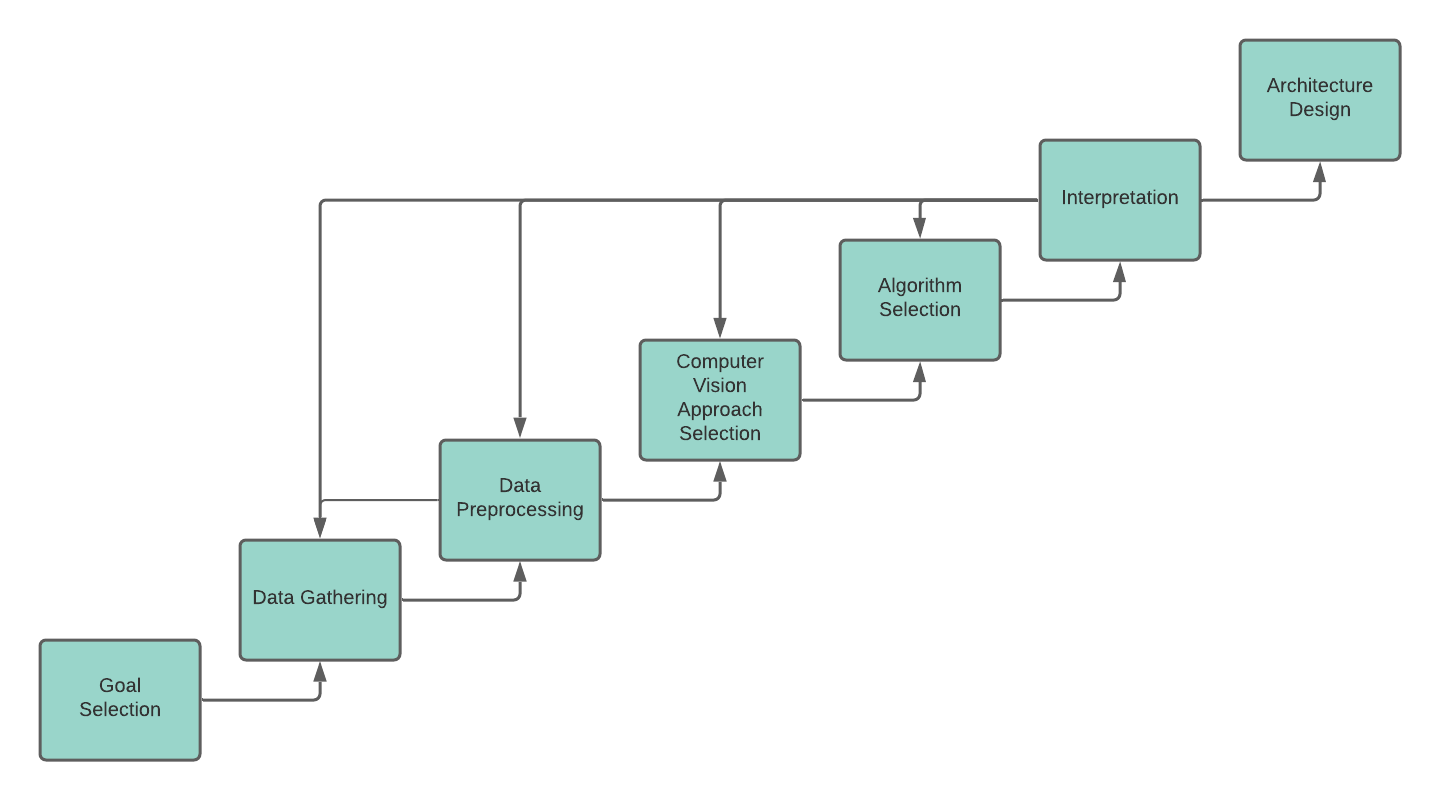
\includegraphics[width=1\textwidth]{images/adapted_development_process.png}
        \caption{Adapted development process from "\citetitle{luckert2016using}", by \textcite{luckert2016using}. Describes the taken steps from data collection, through algorithm selection to architecture design.}
        \label{fig:development_design}
\end{figure}
In this chapter the different steps taken to create a 3D object detector are addressed. 
This chapter adapts the structure proposed for machine learning algorithms proposed by \textcite{luckert2016using}.
The following questions are answered over the course of this chapter:
\begin{itemize}
    \item How can cow teats be recognized?
    \item What are the current method's goals and limits?
    \item What is the method's pipeline composed of?
    \item What is required to apply the method?
\end{itemize}


In order to answer these questions, the structure of this chapter is illustrated as follows: Section \ref{chap:3:goal} describes the first step. It defines the computer vision task and limits its scope. Then, the choice of a suitable data set and the composition of the collected raw data is presented. Section \ref{chap:3:data} describes the information available and the choice of features for the given task. Afterwards, it describes the preprocessing of the data by identifying noise or erroneous inputs. Section \ref{chap:3:method} describes the choice of three proposed processing pipelines and the considered algorithms and techniques.  The interpretation of the performance of the algorithm is described in Section \ref{chap:3:interpretation}. This section also describes how the method results were evaluated, how the algorithms were compared to each other and which parameters were adjusted. Finally, Section \ref{chap:3:architecture} describes the architecture of the processing pipeline, illustrating the diverse components' behaviors, interactions and deployment constraints.
% dacross for determining the 3D position of the salient object. 
% It also sets out the assumptions we took and the choices of technologies with respect to what was discussed in Section 2.

% domain model
%  
\section{Identification of the Computer Vision Goal}\label{chap:3:goal}
The predetermined goal of this project work was to propose a 3D object detection of cow teats solution using machine learning. As mentioned in Section \ref{chap:1:problem}, this project work tackles the following research question: 
\begin{itemize}
    \item How can the cow teats 3D pose be estimated under 10 seconds?
    % \item How can the cow teats 3D pose and direction estimation be evaluated?
\end{itemize}
To answer this question, the following practical steps were laid out:
\begin{itemize}
    \item Conceive a computer vision processing pipeline with optimal prediction quality for identifying the 3D pose and direction of a cow teat.
    \item Present a method for evaluating the quality of the predictions regardless of the method used.
\end{itemize}
This strategy was determined because the steps for data creation and preprocessing are independent of the approach used. Therefore, the remaining task is to propose a machine-learning-enabled pipeline that solves the indicated computer vision task without a priori knowledge of the input system. The main challenge in the processing pipeline is the usage of the diverse types of information the input system provides. The method for evaluating the quality of the predictions will then be built on the results of the processing pipeline. Therefore, the computer vision task is solved by the first step and and the second one is solved by looking at the prediction outputs.

\section{Image Data}\label{chap:3:data}
In order to evaluate computer vision predictions it is essential to gather sufficient quantities of raw data and to layout a simple data structure as required. The following questions will be answered in this section:
\begin{itemize}
    \item What kind of data is necessary?
    \item What kind of structure fulfills the requirements for the present study?
    \item What is the origin of the data?
    \item What are the preprocessing steps?
\end{itemize}
Traditional computer vision tasks require the following types of data: a training data set, for training the algorithm on the domain-specific data and a test set to determine the algorithm's prediction quality. As stated in Section \ref{chap:3:goal}, the given task is to estimate the 3D pose and direction cow teats for a cow milking robot. Therefore, the input data current accessible is: an RGB image, a depth image and a point cloud. The first attempts at tackling the problem using depth images for object classification using traditional computer vision methods failed to meet the performance criteria. Also, under the current project's conditions it is not viable to manually annotate a point cloud. It is also unfeasible to load a batch of point clouds into memory for training. Given the lack of additional inputs, each entry of the data set contains:
% to show any prediction outputs, and the execution time was over 300ms
\begin{itemize}
    \item RGB image of the cow teats.
    \item Pixel-wise segmentation mask, labeling the locations of the cow teats in the RGB image.
\end{itemize}
The nature of the data was two fold: synthetic and realistic. The collection of the realistic data was done at a laboratory at the ZHAW. Given the limitations of the first iteration of the milking robot project, the collection of real cow images was not required. The environment setup and details of the training data collection are described in Chapter \ref{chap:evaluation}. Finally, even though the images collected from the camera could be directly used for training, the preprocessing required was the adaptation of the data set to the COCO data format. Once formatted, the neural network could be trained.

Consequently, the collection of the synthetic data was done using Unreal Engine 4 and a plugin from NVIDIA \cite{2021ue4} called NDDS \cite{2021ndds}. Photorealistic scenes are created in Unreal Engine 4 and NDDS allows for the annotation of objects in UE4. These scenes are then exported and all the information from the objects is included in the export, such as objects, classes and 3D poses. Additionally, the export includes the respective rgb image, depth image, instance segmentations and class segmentations for the frame taken. Appendix \ref{appendix:ndds} illustrates a 3D scene and an export sample.

\section{Specification of a Computer Vision Approach}\label{chap:3:method}

This section describes choice of a computer vision approach for object segmentation, the proposal of 3d pose estimation pipelines and the actual processing step. The following questions will be answered in this section:
\begin{itemize}
    \item Which and how many approaches were considered appropriate for the object segmentation task?
    \item Which and how many approaches were considered appropriate for the pose estimation task?
    \item What optimization steps were taken on the algorithm for the data set?
    \item What were the main problems found during this phase?
\end{itemize}
A trade-off between machine learning techniques is always involved when comparing the advantages and disadvantages of each approach. Therefore, a variety of approaches were considered for the mentioned tasks, evaluated and optimized.

\subsection{Object Segmentation Approaches}

As described in Section \ref{chap:2:segment}, object segmentation involves the pixel-wise assignment of labels in an image that belong to a specific class. The following techniques were considered suitable for this task:
\begin{itemize}
    \item \textbf{Thresholding} A threshold value divides the pixels by intensity value, into background and foreground, generating a binary image.
    \item \textbf{K-Means clustering} A K number of clusters is given to divide the data in to K groups or clusters, based on similarity.
    \item \textbf{Histogram-based image segmentation} A histogram is used to group pixels based on gray levels, where the background is one big peak and then the other "hills" are objects.
    \item \textbf{Edge detection} Changes in brightness are identified using filters to locate edges, curves and shapes. 
    \item \textbf{Convolutional Neural Networks} As described in Section \ref{chap:2:segment}, convolutional operations are used to label the pixels. This approach scans the image by segments, for example using a sliding windows approach.
    \item \textbf{Fully Convolutional Networks} Contrary to to CNNs, FCNs can take different kinds of input, and output a matrix of dimensions H x W x C (image height, image width, number of classes).  
\end{itemize}
Among all the suitable methods tested, the segmentation problem was best tackled using two implementations of MaskRCNN: matterport/MaskRCNN and Detectron2 (FacebookAI). The evaluation and performance of both approaches is described in Section 5.

%As of 28.12.2020, MaskRCNN's repository has not been updated since 01.04.2019 and has over 1500 issues.

\subsection{Pose Estimation Approaches}

As described in Section \ref{chap:2:segment}, object segmentation involves the pixel-wise assignment of labels in an image that belong to a specific class. The following techniques were considered suitable for this task:
\begin{itemize}
    \item \textbf{Recognition of Fixed Shapes} A set of features are generated from the geometric information, such as 3D points, lines or surfaces. These features are then matched to a predefined model features. If the similarity evaluation between the model and the detected features is sufficient, a frame transformation is executed to identify the pose of the detected object. This pose detection represents a hypothesis, among many other hypothesis which are generated while evaluating, for example, a point cloud. Therefore, an appropriate criteria must be used to determine if the hypothesis should be accepted or rejected (hypothesis evaluation). An alternative approach consists of single generating descriptor features from clusters generated in a scene for posterior matching.
    \begin{description}
    \item \textbf{Algorithm Used: } RANSAC \cite{2021scikit-ransac}.
    \end{description}
    
    \item \textbf{Recognition of Object Classes} An algorithm is used to recover a 3D model from the input (image or point cloud), which is then segmented and then classified. Methods like an RDF classifier or CNNs can be used for classification. Then, methods like surface-to-surface distance minimization are used to retrieve the best match. Both realistic and synthetic RGB-D data sets have been published over the past few years for training and testing RGB-D algorithms. Furthermore, it is important that these methods are able to infer the complete 3D shape from a single frame, specially for robotic tasks like grasping.
    \begin{description}
    \item \textbf{Algorithm Used: } DOPE \cite{tremblay2018deep}.
    % \item \textbf{Algorithm Used: } 

    \end{description}
    
    \item \textbf{Feature-based Recognition} Similarly to the recognition of fixed shapes, a set of 3D descriptor features are generated from the geometric information (keypoints) and then evaluated. These descriptor features can be defined by a set of  parameters, such as point coordinates unit vector orientations, point feature histograms of the local surface properties (PFH), etc. A major advantage of these methods is that they require only a single correct feature correspondence to recognize an object.
    \begin{description}
    \item \textbf{Algorithm Used: } Manual Manipulation "MAV". This algorithm leverages the segmentation mask and overlays it over the depth image. Afterwards, the 2D points are proyected into 3D space and PCA is used to calculate the teat direction. Finally, the N points (averaging method) at the bottom of the teat (using the direction indicated by PCA's first component) are averaged to obtain a "teat's tip coordinates". A manual offset was added to the obtained coordinates to attempt to fix the (x,y,z) error observed.
    \end{description}
    
\end{itemize}
\begin{figure}[!ht]
        \centering
        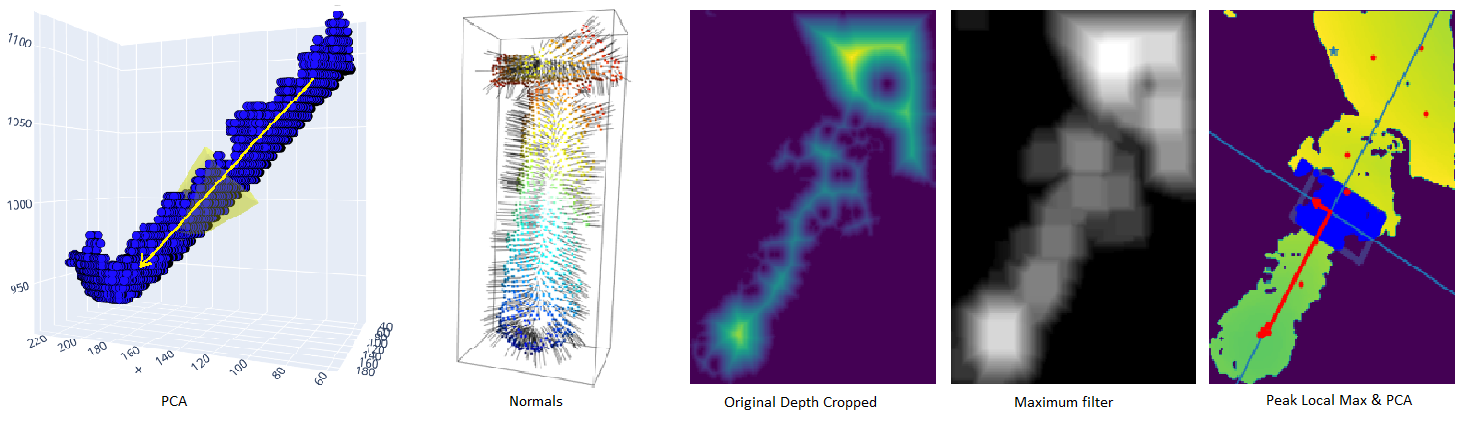
\includegraphics[width=0.8\textwidth]{images/cow_pose_methods.png}
        \caption{Illustration of algorithms to analyze 2D and 3D features. From left to right: PCA in a 3D scatter plot; normals of the points found; 2D erosion to remove outliers, dilation and usage of PCA to find points direction.}
        \label{fig:cow_fmc}
    \end{figure}
For each of the methods described above implementations were chosen to predict based on the data sets.  It is important, during the construction and training of a classifier, to tune the parameters of each model. On one hand, for the object segmentation approach, the parameters that were tuned were the learning rate, the score threshold for prediction, the number of workers, the number of iterations, the images per batch and the batch size. On the other hand, for the pose estimation approaches many parameters were tuned, specific to the method, such as maximum number of cow teats in memory, memory tracking reset conditions, frame transformations, etc.

There were several challenges faced during this phase. Both synthetic and realistic data sets were used for validating not only the models but also the data sets. It was observed that 1) some implementations of the segmentation network used were slower than the final implementation used and 2) the synthetic data set was too different and the reality gap could not be closed. Additionally, allocating resources in the CPU posed a problem in the diverse training and testing. This could be solved by allocating resources in a remote GPU cluster, but set different kind of limitations in the development process.  Finally, due to the fact that many algorithms were tested, the architecture's base concept was a modular design with a plug-and-play approach.

\section{Interpretation}\label{chap:3:interpretation}
%  This section also describes how the method results were evaluated, how the algorithmswere compared to each other and which parameters were adjusted
In order to determine, which implementation of the algorithms work best, a set of metrics need to be taken into consideration to evaluate the outputs of the different algorithms. The metrics are described in Chapter \ref{chap:evaluation} and were used to adjust the data sets and tune both the training and prediction parameters of the algorithms. In the current task there is only one label, so the label distribution is not a challenge. Therefore, a low misclassification rate or respectively a high accuracy rate can be treated as an algorithm result of very high quality \cite{luckert2016using}. On one side, to improve the segmentation algorithm's accuracy, both false positives and false negatives were identified, labelled and added to the data set. On the other side, to improve the pose algorithm's accuracy, different approaches were taken. For example, in the MAV algorithm an offset was calculated and added manually, and an averaging mechanism was added to calculate the cow teat's tip. Subsequently, a correlogram was used to analyze the influence of the camera position and orientation on the error estimation. The correlation coefficients proved a strong indirect correlation and the error showed to be normally distributed. Therefore, linear models are a promising step for predicting and subtracting the error. 
% It is part of the further steps in Chapter \ref{chap:conclusion} to minimize the error offset using a separate algorithm. 
To compare the algorithms among each other, the average error from the errors in (x,y,z) against the cow teat's tip ground truth was evaluated. 

\section{Processing Pipeline}\label{chap:3:architecture}
\begin{figure}[!ht]
        \centering
        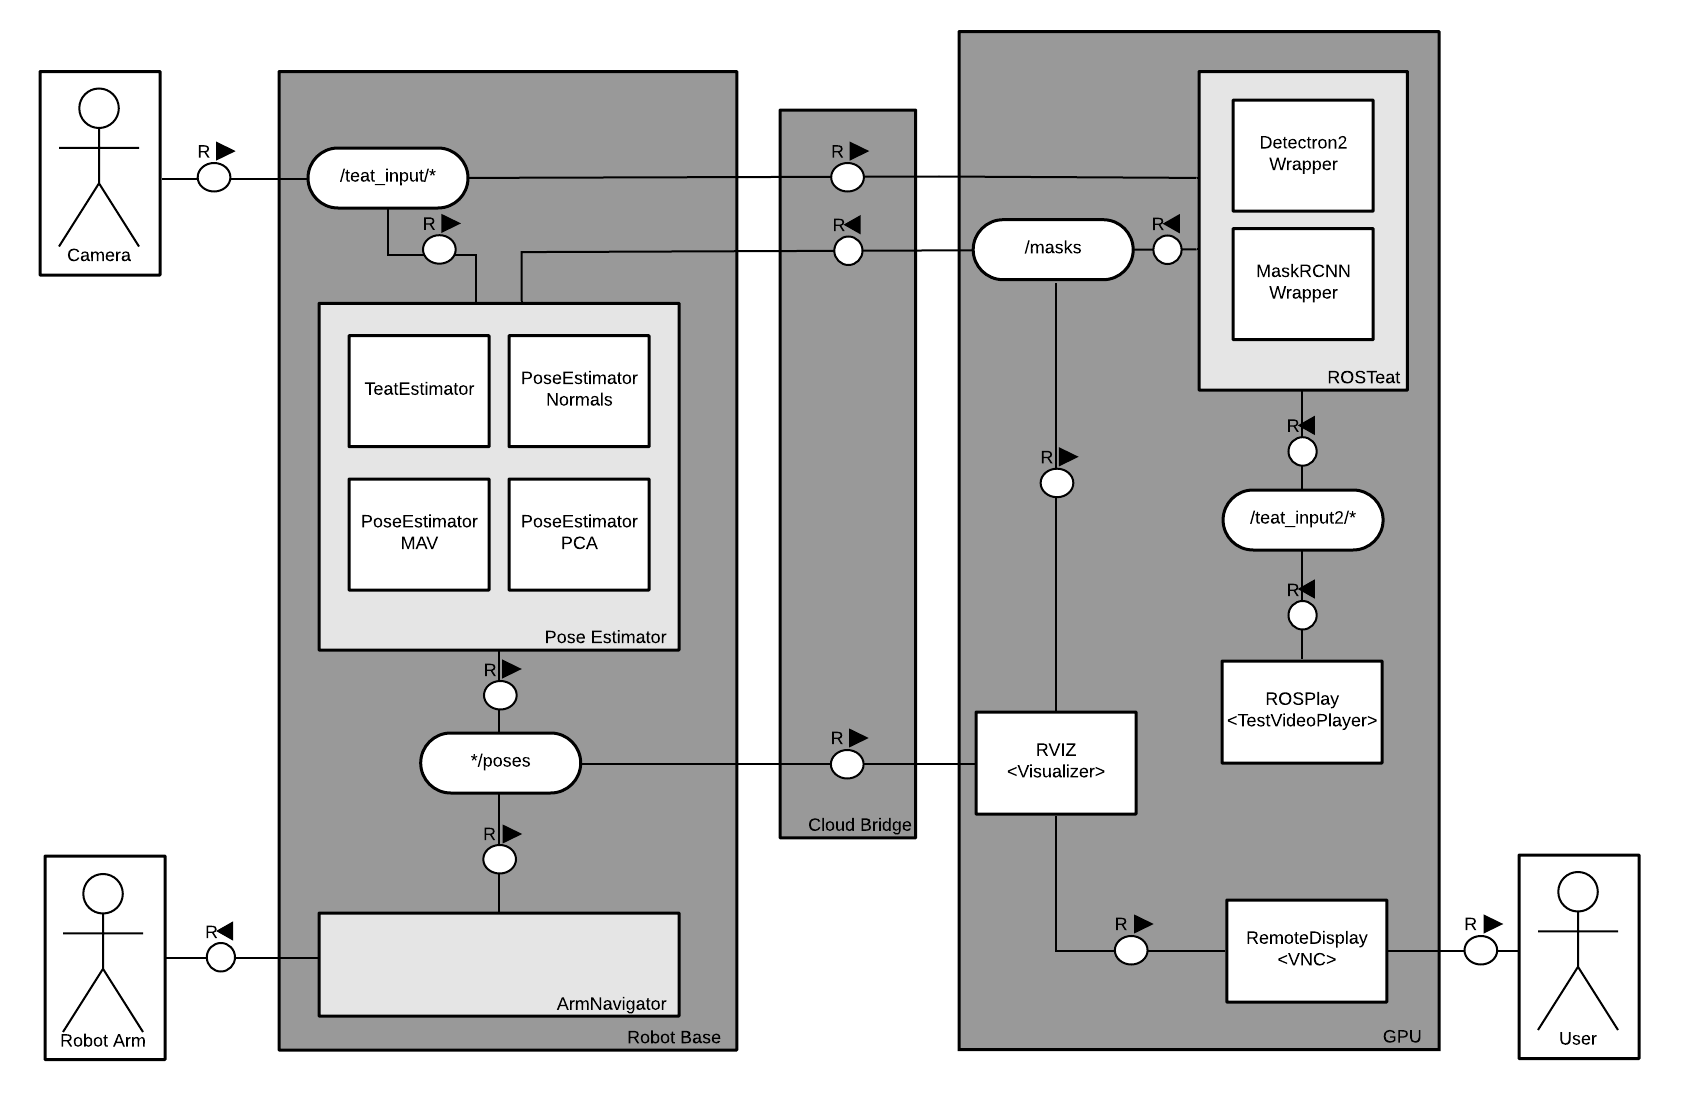
\includegraphics[width=.9\textwidth]{images/cow_fmc.png}
        \caption{FMC diagram of the Pipeline's Architecture}
        \label{fig:cow_fmc}
    \end{figure}
% \section{Software Design} 
% \section{FMC Diagram}
As a tool for designing a modular architecture, a domain model is used to help solve and understand the complexity in the system. The Fundamental Modeling Concepts (FMC) provide a framework for the comprehensive description of software-intensive systems \cite{FMCdiag}. 
% Its block diagrams show the compositional structures as a composition of collaborating system components.
In this framework, active system components are called agents and passive system components are called locations (storage, channels, queues; where information can be observed). The FMC diagram in Figure \ref{fig:cow_fmc} describes the high-level overview of the system's architecture, which illustrates the following agents and locations:
\begin{itemize}
    \item \textbf{Camera:} captures frames and publishes these as input for all the other components.
    \item \textbf{User:} uses Rviz to visualize: the point cloud, the RGB image, the depth image, the segmented image of the cow teats and the 3D poses published.
    \item \textbf{Robot Arm:} moves according to the instructions given by ArmNavigator. 
    \item \textbf{PoseEstimator:} pose estimation algorithm that processes the information received from the camera and ROSTeat to predict 3D poses.
    \item \textbf{ROSTeat Node:} processes images from the Camera node and segments the cow teats in the image.
    \item \textbf{ArmNavigator:} manipulates the RobotArm according to the 3D poses published.
    \item \textbf{ROSPlay <TestVideoPlayer> Node:} Behaves as a simulation/testing mechanism for reproducing the camera videos.
    \item \textbf{RVIZ <Visualizer>:} ROS framework that allows the visualization of different ROS topics (RGB image, point cloud, etc.)
    \item \textbf{RemoteDisplay <VNC>:} this is a browser-based graphical-d
    esktop system that allows the visualization of RVIZ.
    \item \textbf{/teat input/*:} channel where the camera input is published for other components to consume.
    \item \textbf{/teat input2/*:} channel where the simulation video is published as input for other components to consume.
    \item \textbf{/masks:} channel where the segmented cow teats are published.
    \item \textbf{*/poses:} channel wehre the 3D cow teat poses are published.
\end{itemize}
One of the problems that appeared during this phase, was communicating the ROS (Robot Operating System) published messages across two networks. 
% The ROS topics are the buses over which ROS nodes exchange messages (input images, masks, poses, etc.)\cite{2020ROStopics}.
After thorough research it was found that ROS needs a routing mechanism that forwards the published topics (communication buses) from the Robot Base to the GPU and vice versa. The Cloud Bridge uses agents which are deployed on each network, to allow the intercommunication of topic messages. This allowed the deployment of the segmentation network in the GPU cluster, and the pose-estimation-related components in the Robot Base. 
% The behavior and interactions of the main components (ROSTeat and Pose Estimator) are described in the following sections with more detail.

\subsection{Use Cases}
As part of the analysis process, one of the well established fundamental techniques is used: use cases. The use cases identified, which capture the black box requirements requirements for the given task, are 1) cow teat segmentation and 2) pose estimation. The sequence of activities and events described Table \ref{tab:use-segment} and Table \ref{tab:use-pose} takes special conditions and exceptions into consideration.

\begin{longtable}{@{} p{3.5cm} p{10.5cm} @{}} \toprule
\textbf{Use Case}       & \textbf{Segment Cow Teats from Image} \\ \midrule
Actor                   & ROSTeat Node \\ \cmidrule{1-2}
Description             & A cow teat is recognized from an image. \\ \cmidrule{1-2}
Goal                    & Publish the cow teat masks present in received image. \\ \cmidrule{1-2}
Preconditions           & An image exists. \\ 
                        & ROSTeat node is running. \\ \cmidrule{1-2} 
Postconditions          & A number of masks have been identified from image [0+]\\ \cmidrule{1-2} 
                        & 1. The camera publishes an image. \\ 
Basic Flow              & 2. The ROSTeat node consumes the image and predicts the cow teats in it. \\
                        & 3. The ROSTeat node publishes the masks for future processing. \\ \cmidrule{1-2}
Exceptions             & Image is not RGB \\ \bottomrule
\caption{Use Case - Predict Masks} \label{tab:use-segment} \\
\end{longtable}

% \newpage
\begin{longtable}{@{} p{3.5cm} p{10.5cm} @{}} \toprule
\textbf{Use Case}       & \textbf{Estimate 3D Pose of Cow Teat} \\ \midrule
Actor                   & Pose Estimator \\ \cmidrule{1-2}
Description             & A cow teat pose is recognized from a tuple (image, point cloud, depth image, mask). \\ \cmidrule{1-2}
Goal                    & Publish the cow teat poses for each message received. \\ \cmidrule{1-2}
Preconditions           & An image exists. \\ 
                        & ROSTeat node is running. \\ \cmidrule{1-2} 
Postconditions          & A number of cow teat poses have been identified from image [0+]\\ \cmidrule{1-2} 
                        & 1. The camera publishes an image AND ROSTeat node publishes the masks for the image (synchronized receival, stored as a tuple). \\ 
Basic Flow              & 2. The Pose Estimator node consumes the tuple and predicts the cow teat poses in it. \\
                        & 3. The Pose Estimator node publishes the poses for posterior attachment. \\ \cmidrule{1-2}
                        \\
                        \cmidrule{1-2}
Exceptions             & TransformListener is empty \\ 
                       & Any element in the tuple is empty and masks are not (data corruption). \\ \bottomrule
\caption{Use Case - Predict Poses} \label{tab:use-pose} \\
\end{longtable}

\subsection{Design}
Given the nature of the recognition problem, it was determined that it is important to minimize assumptions on poses or camera angles (frame information) and account for the natural variation of the cow teats (udder morphology, colors, light conditions, etc.) as described in Section \ref{chap:2:melkroboter}.
Figure \ref{fig:cow_topics} aids to illustrate a high-level overview of the communication fashion between components.
Finally, given the modular design and message-based principles laid out, allowing any pose estimation algorithm to be used, the pipeline's proposed design is described below:

\begin{enumerate}
    \item The camera publishes information (RGB image, point cloud, depth image) into the input ROS topic channel, which is consumed to identify the position and size of salient objects.
    \item The ROSTeat node subscribes to this input channel, uses the neural network to predict the cow teat masks and publishes them into a masks channel.
    \item The Pose Estimator (plug-and-play component) consumes the masks that were published, and synchronizes it with the camera information (so it is all processed as a single message). The following pose estimation is algorithm-specific. Each pose estimation algorithm is described in detail in the following section. The poses are then published into a poses channel.
    \item The robot consumes messages from the poses channel and moves 10-15 cm forward towards the indicated 3D poses, until it is 20-30 cm close to the pose estimations. Then the attachment process is initiated.
\end{enumerate}

\begin{figure}[!ht]
    \centering
    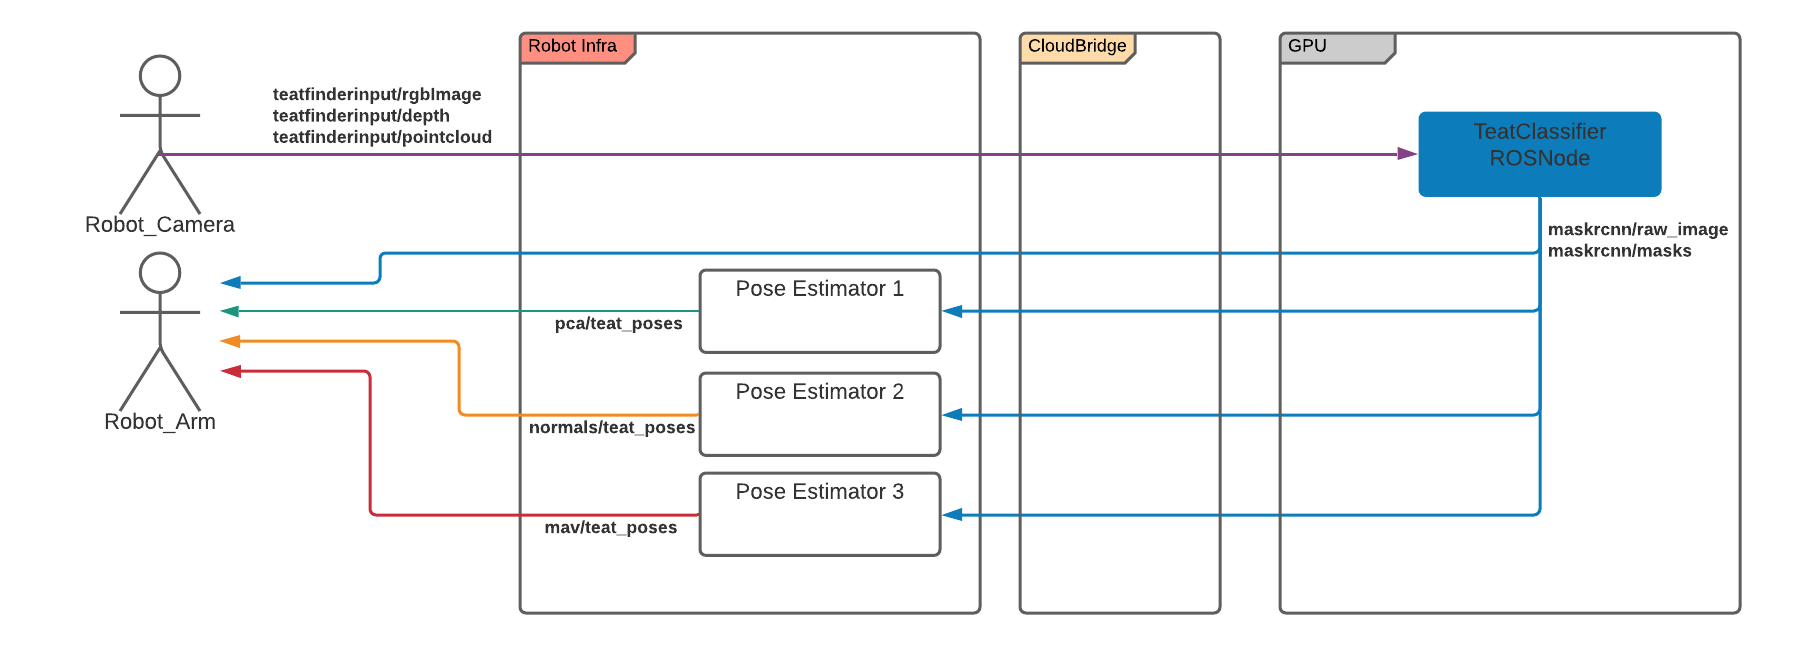
\includegraphics[width=1\textwidth]{images/cow_topics.png}
    \caption{High-level flow diagram of the teat estimation pipeline.}
    \label{fig:cow_topics}
\end{figure}

%  As explained in Section \ref{chap:3:architecture} the messages must go through a Cloud Bridge to be able to connect the robot's ROS local topics with the GPU ROS topics. 


As described above, the interactions between the camera and the recognition components depend on the messages received (images, masks). In order to improve the efficiency of the development process, the ROSPlay component was introduced to allow the repetition of camera frames from a ROSbag (ROS format for a video file). A ROSBag is then used for data generation, algorithm training and testing. One of the problems encountered in this phase was that the generated ROSbags are up to 20 GB in size. These ROSBags are generated in the ROS Base and have to be transferred over the network to the development environment (local laptop or GPU cluster). This can be time consuming but it is required for the development.  
Appendix \ref{appendix:cow_design} additionally provides an alternative illustration for the processing pipeline.